\clearpage
\part{GarmentLab: RGB transfer learning}
\section{Research questions and data protocol}\label{sec:garmentlab}
GarmentLab extends the from-scratch Fashion-MNIST comparison to six-class classification of selected RGB garment crops with an ImageNet-pretrained encoder. It examines encoder adaptation, controlled regularization and confidence-based review. The different label space and data origin are analyzed separately from the ten-class benchmark.

\subsection{Task, preparation and evaluation units}
Fashionpedia supplies instance-level garment annotations \cite{fashionpedia}. Eligible bounding boxes are mapped to six categories: shirt/blouse, top/T-shirt/sweatshirt, jacket, pants, skirt and dress. Each example is one annotated garment crop; the experiment assumes the region has already been selected. Localization and unrestricted full-image recognition are outside this task.

The prepared subset contains 17,827 crops from 12,419 image IDs. Images are decoded as RGB; bounding-box coordinates use floor for the left/top boundary and ceil for the right/bottom boundary. Crops are letterboxed to $224\times224$ with bilinear resizing and black padding, then normalized with ImageNet channel statistics. Nonidentity EXIF orientation is rejected to preserve the relationship between annotation coordinates and decoded pixels. The metadata eligibility filter accepts license IDs 0, 1 and 6; it records source metadata rather than independently establishing usage rights.

\begin{center}\small
\begin{tabular}{lrrrr}\toprule
Category & Fit & Selection & Calibration & Assessment\\\midrule
Shirt/blouse & 1,284 & 180 & 172 & 19\\
Top/T-shirt/sweatshirt & 3,459 & 461 & 448 & 93\\
Jacket & 1,308 & 183 & 159 & 21\\
Pants & 2,398 & 309 & 295 & 49\\
Skirt & 773 & 107 & 116 & 33\\
Dress & 4,605 & 598 & 645 & 112\\\midrule
Total crops & 13,827 & 1,838 & 1,835 & 327\\
Source groups & 9,610 & 1,274 & 1,302 & 221\\
Duplicate components & 9,339 & 1,265 & 1,243 & 221\\\bottomrule
\end{tabular}\end{center}
Source groups merge records with the same source identity; the number of groups can therefore be smaller than the number of image IDs. Exact decoded-image checks and a perceptual-hash graph at Hamming distance two identify additional duplicate components. Within a cross-role component, the highest-priority role is retained and lower-priority source groups are quarantined, in the order assessment, calibration, selection, then fit. No retained source group spans roles. These checks reduce detectable duplication, but a perceptual-hash component is not a verified garment or person identity.

Fit data update weights. Selection data choose checkpoints and recipes. Calibration data determine confidence scaling and the review policy. The 327 assessment crops originate from the separate validation archive and cover only 221 source groups. They are imbalanced, particularly for shirt/blouse and jacket. The original transfer-learning study used assessment after freezing its choices. Because those outcomes were then inspected, the subsequent tuning study treats the same assessment as \emph{post-test exploratory regression evidence}, rather than a new blind evaluation.

\clearpage
\section{Controlled model comparisons}\label{sec:garmentlab-v2}
\subsection{Encoder adaptation and common training settings}
Both baseline recipes use MobileNetV3-Small \cite{mobilenetv3}, initialized with torchvision's \texttt{IMAGENET1K\_V1} weights and a six-output head. The model has 1,524,006 parameters. Frozen-feature training updates only the final linear layer's 6,150 parameters; fine-tuning updates all parameters. Batch-normalization running statistics retain their ImageNet values in both conditions.

The original comparison uses seeds 314, 2718 and 5772, with 18 epochs per recipe and seed. Paired runs share initial head weights and shuffle/flip random streams. Training uses horizontal flips, AdamW, batch size 128, FP32 arithmetic and gradient clipping at 1. The head learning rate is $10^{-3}$; fine-tuning uses backbone learning rate $3\times10^{-4}$, weight decay $10^{-4}$ and head dropout 0.2. A cosine multiplier decays from 1 toward 0.05. Checkpoints maximize selection Macro-F1, breaking ties by lower clean cross-entropy and then the earliest epoch. The deployment seed is fixed at 314.

\subsection{Regularization search and confirmation}
The follow-up retains the architecture, data roles and training budget, and starts each fit from ImageNet initialization. Eight recipes are declared before their discovery scores are computed. Single-factor probes aid interpretation; combined candidates test a recipe without isolating the contribution of each constituent.

\begin{center}\small
\begin{tabular}{llrr}\toprule
ID & Change from fine-tuning anchor & Discovery F1 & Confirmation F1\\\midrule
C0 & Original anchor & 0.84964 & 0.84082\\
C1 & Backbone LR $10^{-4}$ & 0.82535 & --\\
C2 & Weight decay $10^{-3}$ & 0.84643 & --\\
C3 & Label smoothing 0.05 & 0.84868 & --\\
C4 & Head dropout 0.4 & 0.85388 & 0.84245\\
C5 & Brightness/contrast 0.1 each & 0.84995 & 0.84177\\
C6 & C1 + C2 & 0.82494 & --\\
C7 & C1 + C2 + C3 + C4 + C5 & 0.82641 & --\\\bottomrule
\end{tabular}\end{center}
Discovery seed 101 shortlists C4 and C5. The anchor and both challengers are then fitted with fresh seeds 202 and 303. Their mean selection Macro-F1, excluding discovery scores, selects C4. Its advantage over C0 is 0.00162 F1. The same selection images are reused, so fresh training seeds reduce dependence on one initialization without providing an independent validation sample.

C0 and C4 are subsequently trained with final seeds 314, 2718 and 5772. A preset selection-only guard retains the selected seed-314 model unless its F1 regresses by more than 0.005 relative to C0. The observed difference is $-0.00281$, so C4 remains the selected output. Calibration and assessment do not participate in this decision. Label-smoothed training objectives are recorded separately; selection CE is always unsmoothed and evaluated without augmentation.

The follow-up completes $8+6+6=20$ fits and 360 epochs. Recorded fit timers total 4,593.16 seconds; the controller records 5,380.48 seconds including preparation and finalization. Execution used an NVIDIA A100-SXM4-40GB, Python 3.13.16, PyTorch 2.11.0+cu130, torchvision 0.26.0+cu130, NumPy 2.4.2 and CUDA 13.0. Full candidate values, seeds, source bindings and histories are retained in the experiment manifest.

\clearpage
\section{Classification results and training behavior}
\subsection{Encoder adaptation helps; additional tuning does not establish a gain}
The original fine-tuning recipe improves assessment Macro-F1 over frozen features for every paired seed, with gains 0.1182, 0.0773 and 0.0977. This supports adapting the encoder for the prepared subset. The regularization follow-up yields a different conclusion: C4 slightly improves final selection F1 but has lower mean assessment F1 than C0.

\begin{center}\small
\begin{tabular}{lrrrr}\toprule
& \multicolumn{2}{c}{Selection} & \multicolumn{2}{c}{Assessment}\\
Recipe & Accuracy (\%) & Macro-F1 & Accuracy (\%) & Macro-F1\\\midrule
Frozen features & $80.59\pm0.19$ & $0.76220\pm0.00303$ & $74.41\pm0.18$ & $0.67699\pm0.00553$\\
C0 fine-tuning & $87.21\pm0.24$ & $0.84245\pm0.00597$ & $82.06\pm2.25$ & $0.77472\pm0.01493$\\
C4 dropout 0.4 & $87.25\pm0.36$ & $0.84347\pm0.00383$ & $81.75\pm1.16$ & $0.76638\pm0.02258$\\\bottomrule
\end{tabular}\end{center}
Values are means $\pm$ sample SD over three training seeds on fixed partitions; accuracy SD is in percentage points. The C0 follow-up reproduces the original fine-tuning assessment scores. C4's assessment F1 difference from C0 is $-0.00834$. A paired bootstrap jointly resamples the 221 source/duplicate components across both recipes and their three fixed models, using 2,000 replicates and seed 8601. The descriptive 95\% percentile interval for this mean difference is $[-0.03820,+0.01829]$. It includes zero and supports neither superiority nor equivalence. It describes component sampling on this previously inspected assessment, conditional on the fitted models; it does not account for new training seeds or remove selection bias.

\begin{figure}[H]\centering
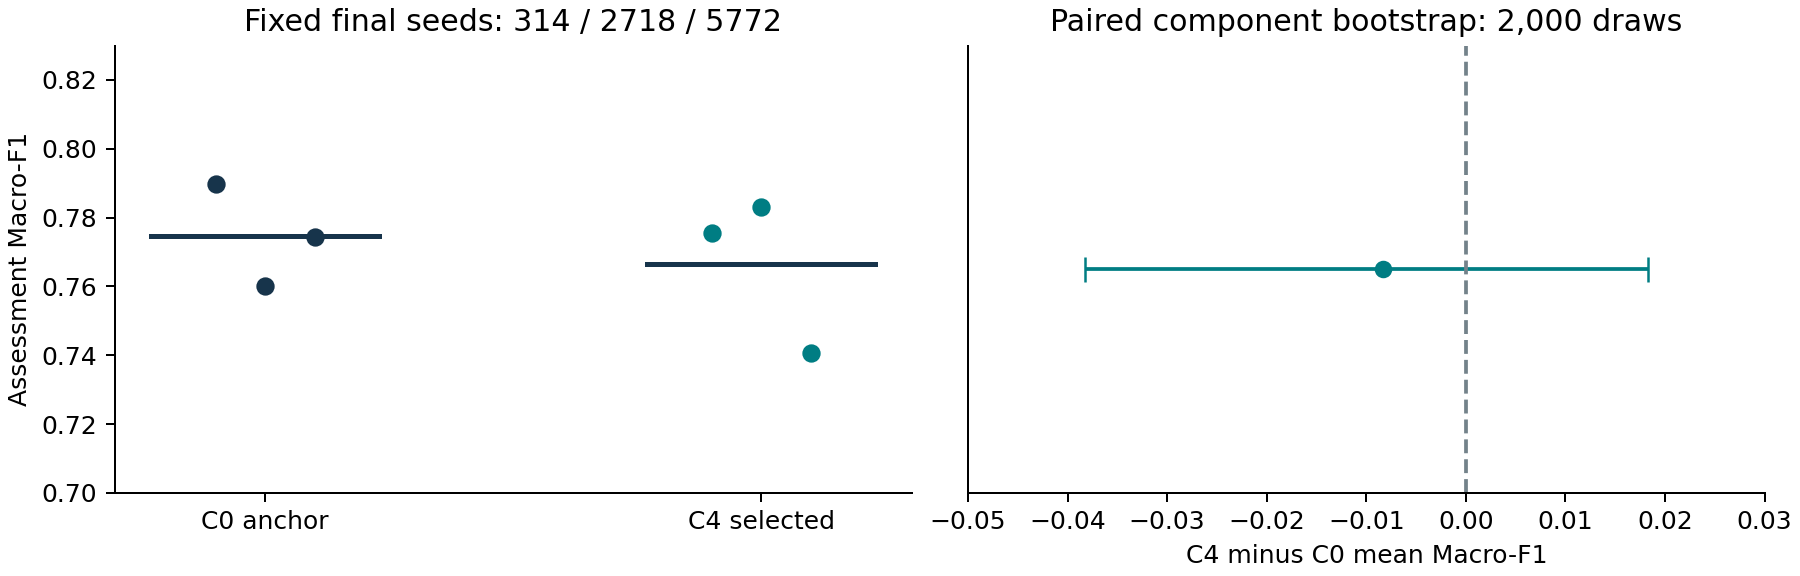
\includegraphics[width=\linewidth]{improve_figures/assessment_comparison.png}
\caption{Final paired assessment results for C0 and C4. Points denote fixed seeds and horizontal marks their means. The interval resamples source/duplicate components jointly rather than treating every crop as independent.}
\label{fig:rgb-paired-assessment}
\end{figure}

\subsection{Overfitting remains visible in loss and accuracy}
For C4 seed 314, training accuracy reaches 99.957\% at epoch 18 while selection accuracy is 87.16\%. Clean selection CE is lowest at epoch 3 (0.42991), then rises to 1.18947 by epoch 18. The F1-selected checkpoint is epoch 17, with selection F1 0.84643 and CE 1.16175. Higher dropout therefore does not eliminate the train--selection gap or excessive raw confidence. Selecting by F1 favors a different objective from minimum CE; each reported row uses metrics from its actual selected checkpoint.

The fixed C4 seed-314 model correctly classifies 269/327 crops (82.26\% accuracy, 0.77553 F1), compared with C0's 274/327 (83.79\%, 0.78989 F1). C4 remains the validation-selected study output, while C0's higher observed assessment score is retained as part of the comparison.

\clearpage
\section{Confidence calibration and selective prediction}
\subsection{Separating probability fitting from threshold selection}
Scalar temperature scaling \cite{temperature} transforms logits $z_k$ into
\[
p_k(x;T)=\frac{\exp(z_k(x)/T)}{\sum_j\exp(z_j(x)/T)},\qquad T\in[0.05,20].
\]
The fitted temperature minimizes calibration NLL. Because $T>0$, scaling preserves class ordering and hence accuracy and Macro-F1. A prediction is accepted automatically when $\max_k p_k(x;T)\ge t$; otherwise it is referred for review. Coverage is the fraction accepted, and accepted accuracy is the correct fraction \emph{within that accepted subset}.

The original C0 procedure fitted temperature and selected an empirical-accuracy threshold on the same calibration partition. The follow-up separates those operations. Joining calibration records by source identity and detected duplicate components produces 1,243 components. A metadata-only split (seed 8401) assigns 621 components, containing 936 crops, to temperature fitting and 622 components, containing 899 crops, to threshold selection. One representative per threshold component is chosen by a seeded hash of annotation identity (seed 8402), before inspecting its logits or label. This avoids counting correlated crops from a component as independent binomial trials and defines an equally weighted representative population.

\subsection{A fixed-grid conditional error bound}
For each threshold in $\{0,0.01,\ldots,1\}$, let $n_t$ and $e_t$ denote accepted representatives and their errors. The one-sided exact Clopper--Pearson upper error limit \cite{exactbinomial} uses significance $0.05/101$. Applying the union bound over the 101 fixed thresholds accounts for selecting a threshold after evaluating the grid. The policy chooses maximum representative coverage among thresholds with $n_t\ge30$ and upper error at most 0.05. If none qualifies, all predictions require review.

For C4, $T=5.345757$ and the selected threshold is $t=0.88$. It accepts 423/622 calibration representatives with six errors, giving 98.58\% empirical accepted accuracy and corrected upper error limit 0.044388. This meets the target \emph{under the binomial assumptions}: a model independent of threshold labels, independent identically distributed representatives, and future data drawn from the same representative population. Historical inspection of calibration, imperfect grouping and deployment shift limit this interpretation. The construction improves data separation and accounts for grid search; it does not supply an unconditional 95\% guarantee for all garment crops or arbitrary photographs.

\begin{figure}[H]\centering
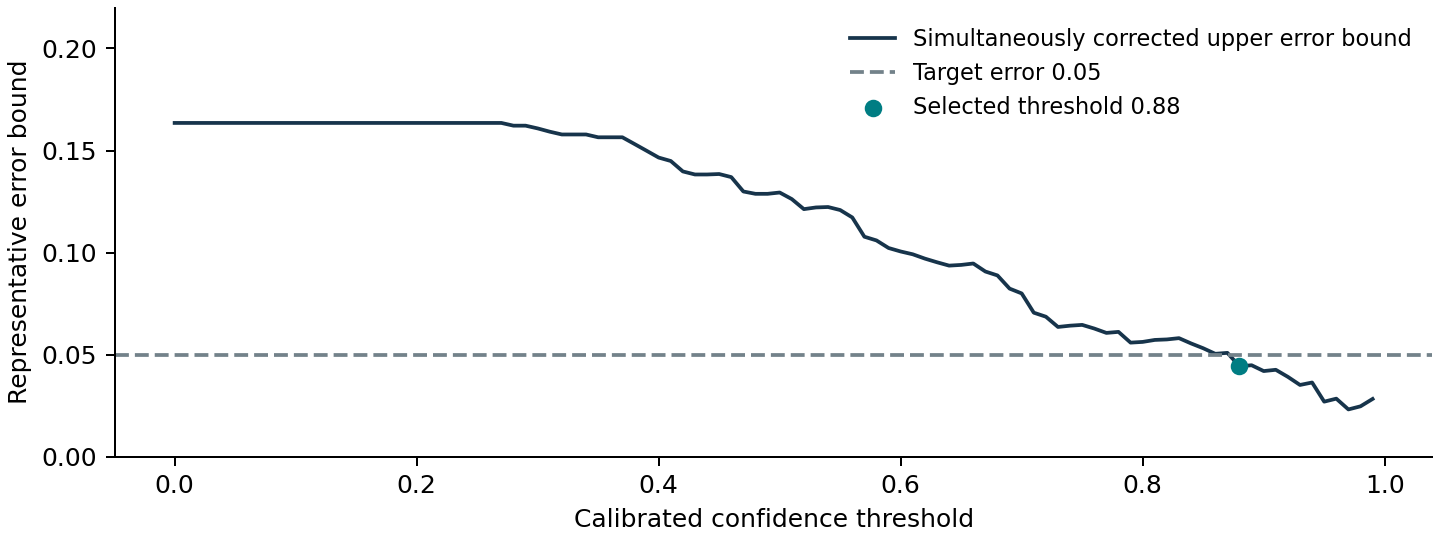
\includegraphics[width=.88\linewidth]{improve_figures/risk_threshold.png}
\caption{Simultaneously corrected upper error limits on the calibration grid, restricted to thresholds accepting at least 30 representatives. The selected threshold 0.88 satisfies the conditional error criterion.}
\label{fig:rgb-risk-bound}
\end{figure}

\clearpage
\section{Reliability, coverage and class-level errors}
\subsection{Calibration changes confidence rather than labels}
Temperatures and thresholds are frozen before assessment inference. Both selected models are overconfident before scaling. NLL and Brier decrease after calibration, while the choice between the calibrated models depends on the metric: C4 has lower ECE but higher NLL than C0.

\begin{center}\small
\begin{tabular}{lrrrr}\toprule
& \multicolumn{2}{c}{C0 seed 314} & \multicolumn{2}{c}{C4 seed 314}\\
Assessment metric & Raw & Calibrated & Raw & Calibrated\\\midrule
Accuracy (\%) & 83.79 & 83.79 & 82.26 & 82.26\\
Macro-F1 & 0.78989 & 0.78989 & 0.77553 & 0.77553\\
NLL & 1.3571 & 0.4843 & 1.5879 & 0.5159\\
Brier score & 0.2899 & 0.2487 & 0.3300 & 0.2618\\
ECE, 15 bins & 0.1339 & 0.0623 & 0.1536 & 0.0499\\\bottomrule
\end{tabular}\end{center}
Brier is the mean sum of squared probability errors across six classes, without division by six. ECE summarizes a particular finite-sample binning and can disagree with proper scoring rules such as NLL and Brier.

\begin{center}\small
\begin{tabular}{lrrrrr}\toprule
Frozen policy & $T$ & Threshold & Correct/accepted & Coverage (\%) & Accepted acc. (\%)\\\midrule
C0, original & 4.922505 & 0.782914 & 211/228 & 69.72 & 92.54\\
C4, disjoint calibration & 5.345757 & 0.88 & 173/182 & 55.66 & 95.05\\\bottomrule
\end{tabular}\end{center}
The C4 policy refers 145 of 327 assessment crops for review. Its accepted-accuracy point estimate is higher than C0's, while coverage falls by 14.07 percentage points and full-sample accuracy is lower. Model and calibration procedure both change between these rows, so the table describes a combined policy outcome rather than isolating a calibration effect. The crop-weighted assessment proportion also differs from the representative-weighted target of the calibration bound.

\subsection{The weakest class is not resolved by tuning}
\begin{center}\small
\begin{tabular}{lrrrr}\toprule
Category & Support & C4 recall (\%) & C0 F1 & C4 F1\\\midrule
Shirt/blouse & 19 & 47.37 & 0.5625 & 0.5806\\
Top/T-shirt/sweatshirt & 93 & 83.87 & 0.8223 & 0.8000\\
Jacket & 21 & 76.19 & 0.8000 & 0.7619\\
Pants & 49 & 87.76 & 0.8980 & 0.8866\\
Skirt & 33 & 66.67 & 0.7667 & 0.7458\\
Dress & 112 & 90.18 & 0.8899 & 0.8783\\\bottomrule
\end{tabular}\end{center}
C4 correctly identifies nine of 19 shirt/blouse crops, with another nine predicted as top/T-shirt/sweatshirt. Dress-to-top confusion contributes nine further errors; six of 33 skirts are classified as dress. These counts identify concrete class boundaries for further analysis. Similar appearance, occlusion, neighboring garments and crop background are plausible contributors, but the experiments do not isolate their causal effects. Small class supports limit the precision of the per-class estimates.

\clearpage
\section{Robustness under fixed perturbations}
The stress suite applies nine predetermined perturbations to already letterboxed assessment arrays. Both checkpoints and their calibration policies remain fixed. Gaussian noise uses standard deviations 0.02, 0.05 and 0.10; blur uses radii 0.5, 1 and 2 pixels; translation uses offsets of 2, 4 and 8 pixels. These synthetic conditions probe specific sensitivities and are not a separate natural-shift dataset.

\begin{center}\small
\begin{tabular}{lrrrr}\toprule
Condition & C0 Macro-F1 & C4 Macro-F1 & C4 coverage (\%) & C4 accepted acc. (\%)\\\midrule
Clean & 0.7899 & 0.7755 & 55.66 & 95.05\\
Noise, $\sigma=0.02$ & 0.7490 & 0.7098 & 51.68 & 94.67\\
Noise, $\sigma=0.05$ & 0.6588 & 0.6711 & 42.81 & 92.86\\
Noise, $\sigma=0.10$ & 0.5512 & 0.6044 & 28.44 & 89.25\\
Blur, radius 0.5 px & 0.7930 & 0.7685 & 55.05 & 94.44\\
Blur, radius 1 px & 0.6952 & 0.7027 & 50.76 & 92.17\\
Blur, radius 2 px & 0.5869 & 0.5941 & 34.86 & 87.72\\
Translation, 2 px & 0.7849 & 0.7279 & 51.38 & 95.24\\
Translation, 4 px & 0.7678 & 0.7418 & 51.68 & 94.67\\
Translation, 8 px & 0.7618 & 0.7825 & 48.62 & 94.34\\\bottomrule
\end{tabular}\end{center}
Strong noise and blur reduce C4 F1 to 0.6044 and 0.5941, decreases of 0.1711 and 0.1814 from its clean result. Although C4 exceeds C0 under these two severe conditions, the relative performance is mixed across the suite. The result is therefore sensitivity to specific perturbations rather than a general robustness advantage for dropout 0.4.

Selective prediction also degrades under these shifts. At the strongest noise and blur settings, accepted accuracy falls to 89.25\% and 87.72\%, despite coverage shrinking to 28.44\% and 34.86\%. Observed accepted accuracy is below 95\% in these conditions; the calibration bound does not certify shifted input populations. Translation results are not monotonic: an eight-pixel shift slightly improves C4 F1 on this finite subset. This can arise from changes in individual crop predictions and does not demonstrate that larger displacement generally helps recognition.

\subsection{What the results support}
The original paired comparison provides consistent evidence that encoder adaptation improves this subset over frozen features. The follow-up does not establish an additional assessment F1 improvement from its selected regularization recipe. Temperature scaling reduces overconfidence, and the stricter selected policy yields higher observed accepted accuracy at lower coverage. Neither regularization nor selective prediction removes the observed class imbalance, overfitting and shift sensitivity.

The distinction between these outcomes matters: a better validation score is not necessarily a better assessment score; a lower ECE is not necessarily a lower NLL; and high accepted accuracy can coexist with lower overall accuracy and substantial human-review workload. Each conclusion concerns its measured population and metric.

\clearpage
\section{Numerical verification and local service behavior}
\subsection{PyTorch execution and ONNX export}
The service processes one selected RGB garment region using the same decoding, crop, letterbox and normalization policy as evaluation. Its release binds weights, label order, preprocessing and calibration parameters. Seven prepared-crop PNG cases exercise the actual image-processing and prediction path; six in-process HTTP checks cover discovery, valid accept/review predictions and invalid-input behavior. Numerical comparisons use a fixed maximum absolute logit tolerance of $10^{-4}$.

\begin{center}\small
\begin{tabular}{p{.43\linewidth}p{.30\linewidth}r}\toprule
Comparison & Recorded cases and batches & Maximum error\\\midrule
C4 PyTorch CPU vs. archived Colab & 327 cases; 1, 3, 64, 128 & $<5.92\times10^{-5}$\\
C4 ONNX, original check & 64 cases; 1, 3, 64 & $9.1970\times10^{-5}$\\
C4 ONNX, expanded check & 327 cases; 1, 3, 64, 128 & $1.3542\times10^{-4}$\\\bottomrule
\end{tabular}\end{center}
The PyTorch comparisons pass, with no label or review-decision differences. The expanded ONNX check fails the fixed numerical tolerance despite matching discrete decisions. Three further CPU exporter/runtime variants also fail that broader criterion. The verified local service consequently uses PyTorch; the ONNX artifact remains experimental. The original 64-case pass and the broader failure are both retained in the evidence.

The CPU checks use Windows, Python 3.12 and PyTorch 2.10, compared with Colab Linux and PyTorch 2.11 for the training return. They test this recorded platform change on the archived cases.

\subsection{End-to-end local HTTP measurement}
A real-server test uses two recorded source JPEG/crop cases, ten warmup requests per supported-concurrency phase and 120 timed predictions each at concurrency one and two. All 240 predictions return HTTP 200. A separate 60.014-second run at concurrency two completes 5,312/5,312 successful predictions: p50 21.70\,ms, p95 31.43\,ms and p99 36.93\,ms, with 88.51 successful predictions/s. Client timing includes multipart construction, loopback transfer, decoding, preprocessing, forward execution and response serialization; source-file reads precede timing.

A 24-request overload probe at concurrency eight produces nine successful predictions and 15 expected busy responses, with no unexpected failures. Invalid-input tests return the recorded 400, 400, 415 and 413 statuses. Successful-prediction throughput is kept separate from attempted requests and overload responses. This short, repeated-input loopback experiment characterizes the local service, not hosted availability or production capacity.

\subsection{Reproducibility and extension conclusion}
The record retains data roles, candidate values, 20 histories, checkpoint decisions, predictions and source bindings. Its audit verifies 273 payload hashes and reconstructs classification metrics, temperature, all 101 threshold bounds and the component bootstrap. A clean isolated environment passes 261 software tests with two condition-dependent skips.

Paired evidence supports encoder adaptation on this subset. Subsequent regularization does not establish a further F1 gain, while calibration trades coverage for higher observed accepted accuracy. Class errors, shift sensitivity and ONNX numerical failure remain. Section~\ref{sec:prospective-followup} reports a later locked cohort from previously unused source groups. Broader service and external-population testing remain necessary for operational conclusions.
